\chapter{Electrons temperature distribution for MMO with }
\label{sec:appendixB}

In this appendix, we plot the normalized velocity component distribution and normalized speed distribution for Case 8. The plots show the distribution at timestep 1,000 when the charging of the MMO has begun to stabilize and converge to the floating potential. The filled in orange sections show the binned particle distribution, while the blue lines show the normalized theoretical Gaussian distribution curves. Figure \ref{fig:appendixBFullDomain} shows the distribution for the whole domain. Due to the large amount of particles in the whole domain, every hundreth electron was included for a total of $1.47 \times 10^6$ particles. From \ref{fig:appB_FD_speed}, it is apparent that the distribution contains a mixture of two electron distributions; the ambient photoelectrons with a higher average temperature, and the photoelectrons. Figure \ref{fig:appendixBPartialDomain} shows the normalized distributions only for particles close to the sunlit spacecraft surface. Note in figure \ref{fig:appB_PD_speed} the lower average temperature of of electrons close to the spacecraft surfaces.


%FULL DOMAIN ELECTRONS
\begin{figure}[H]
  \centering
  \begin{subfigure}[b]{0.75\textwidth}
  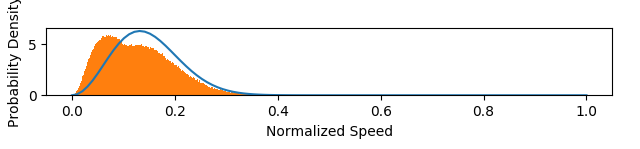
\includegraphics[width=\columnwidth]{figures/Appendix/AppendixB/FD/speedElectrons.png}
  \caption{Normalized distribution of speed of electrons}
  \label{fig:appB_FD_speed}
\end{subfigure}

\begin{subfigure}[b]{0.75\textwidth}
  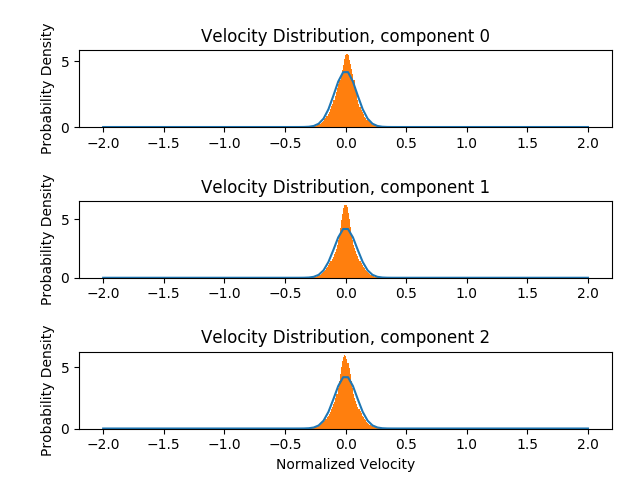
\includegraphics[width=\columnwidth]{figures/Appendix/AppendixB/FD/vel.png}
  \caption{Normalized distribution of velocity components of electrons}
  \label{fig:appB_FD_vel}
\end{subfigure}
\label{fig:appendixBFullDomain}
\caption{Normalized distributions for both speed and velocity components in the whole computational domain}
\end{figure}
% %FULL DOMAIN IONS
% \begin{figure}[H]
%   \centering
%   \begin{subfigure}[b]{0.75\textwidth}
%   \includegraphics[width=\columnwidth]{figures/Appendix/AppendixB/FD/velIons.png}
%   \caption{}
%   \label{fig:}
% \end{subfigure}
% \hfill
% \begin{subfigure}[b]{0.75\textwidth}
%   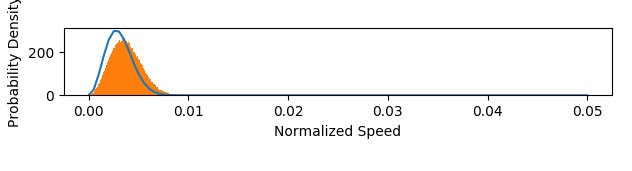
\includegraphics[width=\columnwidth]{figures/Appendix/AppendixB/FD/speedIons.png}
%   \caption{ }
%   \label{fig:}
% \end{subfigure}
% \caption{Dummy}
% \label{fig:}
% \end{figure}

%PARTIAL DOMAIN, ELECTRONS
\begin{figure}[H]
  \centering
  \begin{subfigure}[b]{0.75\textwidth}
  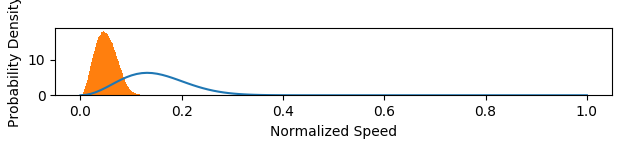
\includegraphics[width=\columnwidth]{figures/Appendix/AppendixB/PD/speedElectrons.png}
  \caption{Normalized distribution of velocity components for electrons close to the sunlit spacecraft surfaces}
  \label{fig:appB_PD_speed}
\end{subfigure}

\begin{subfigure}[b]{0.75\textwidth}
  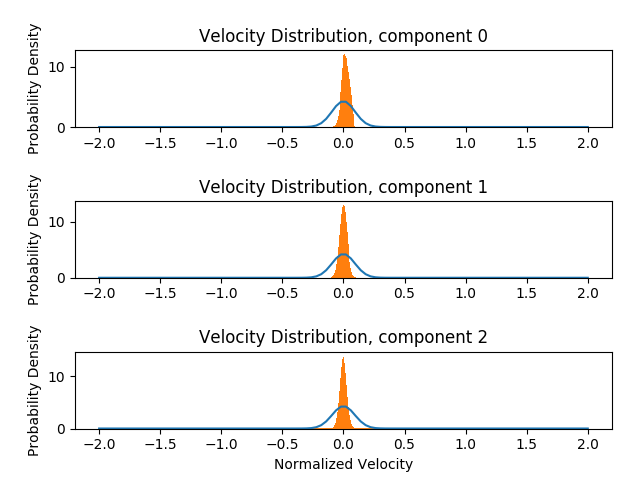
\includegraphics[width=\columnwidth]{figures/Appendix/AppendixB/PD/vel.png}
  \caption{Normalized distribution of speed for electrons close to the sunlit spacecraft surfaces}
  \label{fig:appB_PD_vel}
\end{subfigure}
\caption{Normalized distributions for both speed and velocity components for particles close to the spacecraft sunlit surfaces}
\label{fig:appendixBPartialDomain}
\end{figure}
% %PARTIAL DOMAIN, IONS
% \begin{figure}[H]
%   \centering
%   \begin{subfigure}[b]{0.75\textwidth}
%   \includegraphics[width=\columnwidth]{figures/Appendix/AppendixB/PD/velIons.png}
%   \caption{}
%   \label{fig:}
% \end{subfigure}
% \hfill
% \begin{subfigure}[b]{0.75\textwidth}
%   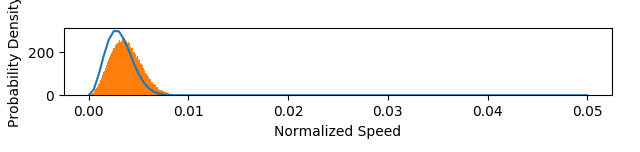
\includegraphics[width=\columnwidth]{figures/Appendix/AppendixB/PD/speedIons.png}
%   \caption{ }
%   \label{fig:}
% \end{subfigure}
% \caption{Dummy}
% \label{fig:}
% \end{figure}